\chapter{Thử nghiệm và kết quả}\label{chapter_experiment}

\section{Thiết lập thí nghiệm}

Phần này trình bày chi tiết cách thiết lập các thí nghiệm để đảm bảo tính công bằng (fairness), tính tái lập (reproducibility) và tính khoa học trong đánh giá mô hình.

\subsection{Chia dữ liệu (Train/Test Split)}

Tập dữ liệu gồm 920 mẫu được chia theo tỷ lệ \textbf{80/20} sử dụng phương pháp \textbf{Stratified Split} với \texttt{random\_state = 42}:
\begin{itemize}
    \item \textbf{Tập huấn luyện (Train set):} 736 mẫu ($\sim$80\%) -- dùng để train mô hình và áp dụng SMOTE.
    \item \textbf{Tập kiểm tra (Test set):} 184 mẫu ($\sim$20\%) -- chỉ dùng để đánh giá cuối cùng, \textbf{không được sử dụng trong bất kỳ bước training nào}.
\end{itemize}

Stratified split đảm bảo tỷ lệ lớp bệnh/không bệnh (55:45) được giữ nguyên trong cả hai tập. Điều này quan trọng vì nếu chia ngẫu nhiên đơn thuần, tập test có thể có tỷ lệ lớp khác biệt đáng kể so với tập train, dẫn đến đánh giá không chính xác. Với \texttt{random\_state = 42}, phép chia là deterministic -- chạy lại sẽ cho cùng kết quả, giúp các thành viên trong nhóm và người đọc tái tạo chính xác kết quả.

Tỷ lệ 80/20 được chọn vì: (1) Với 920 mẫu, tập test cần đủ lớn ($\geq$ 100 mẫu) để đánh giá có ý nghĩa thống kê; (2) Tập train cần đủ lớn để các mô hình phức tạp (XGBoost, Random Forest) không bị underfitting; (3) Tỷ lệ 80/20 là tiêu chuẩn phổ biến trong Machine Learning cho tập dữ liệu kích thước trung bình.

\subsection{Cross-Validation}

Ngoài đánh giá trên tập test (hold-out), nhóm thực hiện \textbf{5-Fold Stratified Cross-Validation} trên toàn bộ dữ liệu để đánh giá tính ổn định (stability) của mô hình. Quy trình: dữ liệu được chia thành 5 fold có kích thước tương đương, mỗi lần sử dụng 1 fold làm tập validation và 4 fold còn lại làm tập training. Quá trình lặp lại 5 lần, mỗi fold được dùng làm validation đúng 1 lần.

Cross-validation cung cấp hai thông tin quan trọng mà hold-out evaluation không có:
\begin{itemize}
    \item \textbf{Mean F1:} Ước lượng performance kỳ vọng, ít phụ thuộc vào cách chia dữ liệu cụ thể.
    \item \textbf{Std F1:} Đo lường variance -- mô hình có Std cao cho thấy performance không ổn định, phụ thuộc nhiều vào dữ liệu cụ thể. Trong y tế, mô hình ổn định (Std thấp) được ưu tiên hơn mô hình có mean cao nhưng variance lớn.
\end{itemize}

\subsection{Thiết lập môi trường thử nghiệm}

Tất cả thử nghiệm được thực hiện với cấu hình nhất quán:
\begin{itemize}
    \item \textbf{Random seed:} 42 cho tất cả các bước (split, SMOTE, KMeans initialization, model training) -- đảm bảo reproducibility hoàn toàn.
    \item \textbf{StandardScaler:} fit trên train set, transform cả train và test -- ngăn data leakage.
    \item \textbf{SMOTE:} áp dụng trên train set sau khi scale -- tạo mẫu tổng hợp cân bằng lớp, chỉ trên train để test không bị ảnh hưởng.
    \item \textbf{Thư viện:} scikit-learn 1.3+, xgboost 2.0+, mlxtend 0.23+, Python 3.10+.
    \item \textbf{Metric chính:} F1-Score (scoring function cho cross-validation), PR-AUC và ROC-AUC (đánh giá trên test).
\end{itemize}

\section{Kết quả khai phá luật kết hợp (Association Rules)}

\subsection{Kết quả tổng quan}

Thuật toán Apriori với tham số \texttt{min\_support = 0.08}, \texttt{min\_confidence = 0.50}, \texttt{min\_lift = 1.2} sinh ra tổng cộng \textbf{3.792 luật kết hợp} từ dữ liệu đã rời rạc hóa. Trong đó, các luật có consequent (kết luận) là ``heart\_disease'' (liên quan trực tiếp đến bệnh tim) được lọc riêng để phân tích. Bảng \ref{tab:top_rules} trình bày 10 luật có confidence (độ tin cậy) cao nhất:

\begin{table}[H]
\centering
\caption{Top 10 luật kết hợp liên quan đến bệnh tim (sắp xếp theo confidence giảm dần).}
\label{tab:top_rules}
\small
\begin{tabular}{|c|p{6cm}|c|c|c|}
\hline
\textbf{STT} & \textbf{Antecedents (Tổ hợp triệu chứng)} & \textbf{Support} & \textbf{Confidence} & \textbf{Lift} \\ \hline
1 & oldpeak\_high, cp\_asymptomatic, slope\_flat, is\_male & 0.0913 & 0.9655 & 1.7451 \\ \hline
2 & exercise\_angina, oldpeak\_high, slope\_flat, is\_male & 0.0837 & 0.9625 & 1.7397 \\ \hline
3 & exercise\_angina, oldpeak\_high, cp\_asymptomatic, slope\_flat & 0.0804 & 0.9610 & 1.7370 \\ \hline
4 & oldpeak\_high, cp\_asymptomatic, slope\_flat & 0.1000 & 0.9583 & 1.7322 \\ \hline
5 & oldpeak\_high, ecg\_abnormal, slope\_flat, is\_male & 0.0913 & 0.9545 & 1.7253 \\ \hline
6 & exercise\_angina, oldpeak\_high, slope\_flat & 0.0891 & 0.9535 & 1.7234 \\ \hline
7 & oldpeak\_high, ecg\_abnormal, is\_male, cp\_asymptomatic & 0.0967 & 0.9468 & 1.7113 \\ \hline
8 & exercise\_angina, oldpeak\_high, is\_male & 0.1130 & 0.9455 & 1.7089 \\ \hline
9 & exercise\_angina, oldpeak\_high, ecg\_abnormal, is\_male & 0.0924 & 0.9444 & 1.7071 \\ \hline
10 & exercise\_angina, oldpeak\_high, cp\_asymptomatic & 0.1076 & 0.9429 & 1.7042 \\ \hline
\end{tabular}
\end{table}

\subsection{Diễn giải y khoa các luật kết hợp}

Phân tích các luật mạnh nhất cho thấy một số pattern y khoa đáng chú ý:

\textbf{Luật 1 (confidence 96.6\%):} Bệnh nhân \textit{nam giới} có \textit{ST depression cao} ($\geq$ 2 mm), \textit{đau ngực không triệu chứng} (asymptomatic) và \textit{đoạn ST phẳng} khi gắng sức $\rightarrow$ nguy cơ bệnh tim cực kỳ cao. Tổ hợp này xuất hiện ở 9.13\% bệnh nhân (84 người), và 96.6\% trong số họ bị bệnh tim. Nguy cơ cao gấp 1.75 lần so với trung bình toàn bộ dataset. Đây là ``hồ sơ nguy cơ'' rõ ràng nhất mà hệ thống phát hiện, phù hợp với kiến thức y khoa: đau ngực ``im lặng'' (asymptomatic) kết hợp bất thường điện tâm đồ là dấu hiệu điển hình của bệnh mạch vành thầm lặng ở nam giới.

\textbf{Luật phổ biến nhất (support 11.3\%):} Tổ hợp \texttt{exercise\_angina, oldpeak\_high, is\_male} (luật 8) xuất hiện ở 104 bệnh nhân -- luật phổ biến nhất trong top 10. Đáng chú ý, chỉ cần 3 yếu tố đơn giản (nam, đau ngực khi vận động, ST depression cao) đã đủ để dự đoán bệnh tim với confidence 94.6\%.

\textbf{Đặc trưng xuất hiện nhiều nhất:} Phân tích tần suất xuất hiện trong top 10 luật: \texttt{oldpeak\_high} (10/10 luật), \texttt{is\_male} (8/10), \texttt{exercise\_angina} (7/10), \texttt{slope\_flat} (6/10), \texttt{cp\_asymptomatic} (6/10). Điều này khẳng định vai trò then chốt của ST depression, giới tính nam và đau thắt ngực khi vận động trong dự đoán bệnh tim -- phù hợp với y văn quốc tế.

\textbf{Ý nghĩa lâm sàng:} Các luật này có thể được sử dụng như ``checklist'' sàng lọc nhanh: nếu bệnh nhân nam trên 55 tuổi có ST depression $\geq$ 2 mm và đau ngực khi vận động, nên ưu tiên xét nghiệm chuyên sâu (chụp mạch vành) để xác nhận chẩn đoán.

\section{Kết quả phân cụm (Clustering)}

\subsection{Xác định số cụm tối ưu}

Nhóm khảo sát số cụm $k$ từ 2 đến 10 sử dụng hai phương pháp bổ sung. Hình \ref{fig:elbow_sil} trình bày Elbow plot (đồ thị inertia) và Silhouette Score theo $k$:

\begin{figure}[H]
    \centering
    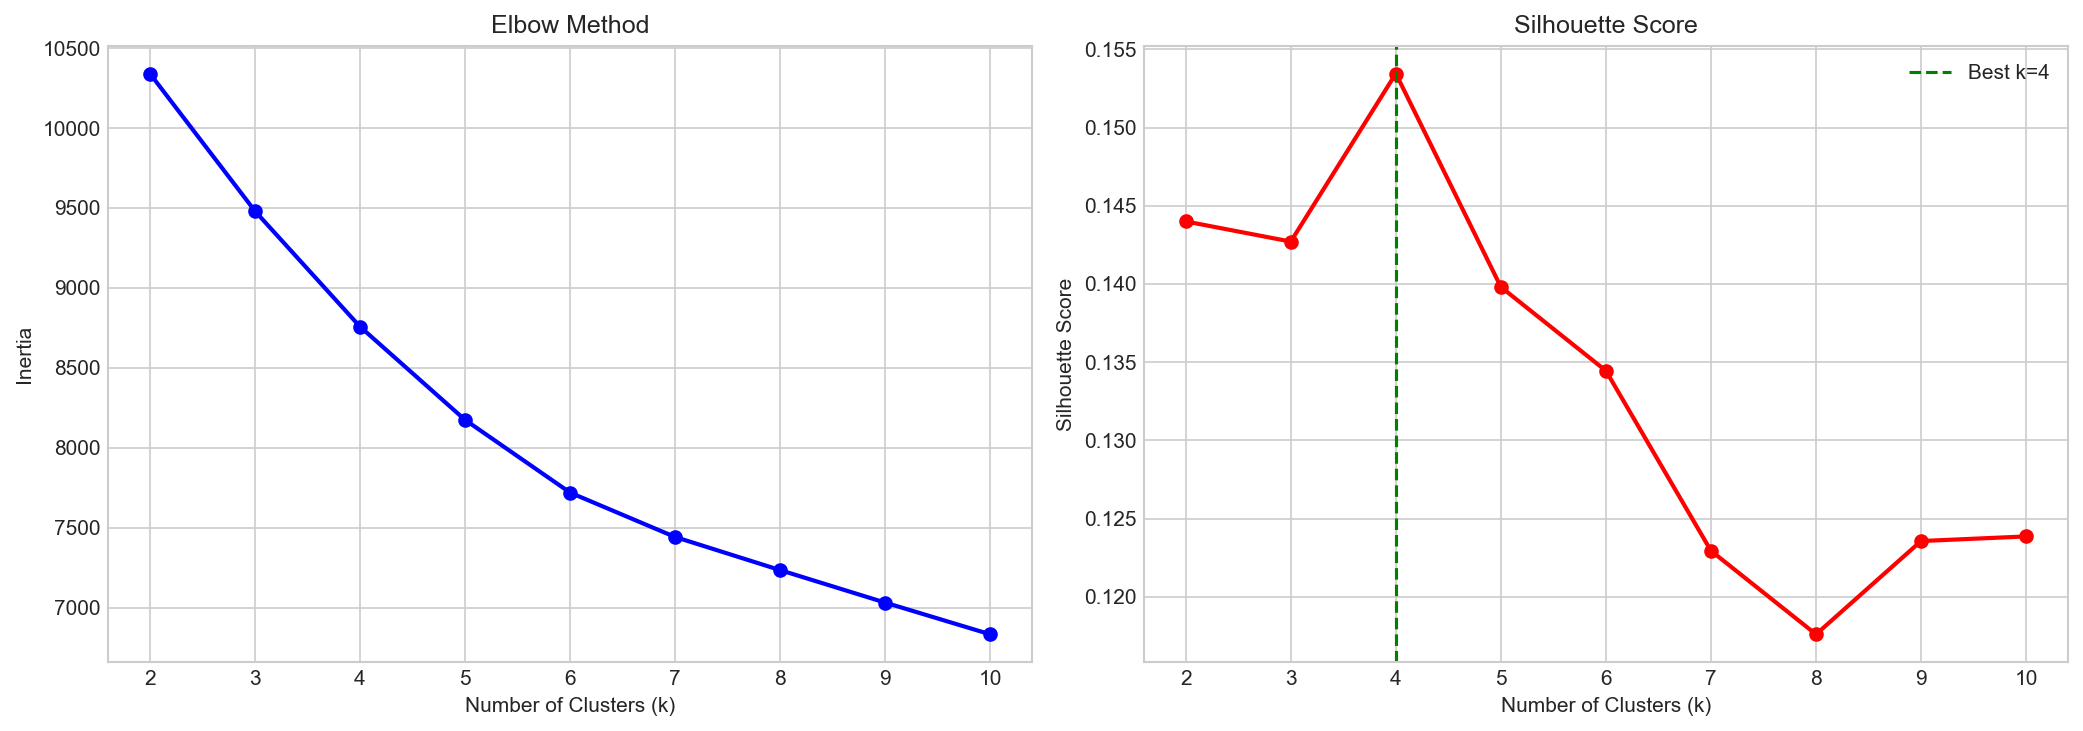
\includegraphics[width=\textwidth]{figs/elbow_silhouette.png}
    \caption{Elbow plot (trái) và Silhouette Score (phải) theo số cụm $k$ -- số cụm tối ưu $k = 4$.}
    \label{fig:elbow_sil}
\end{figure}

Elbow plot cho thấy inertia giảm nhanh từ $k=2$ đến $k=4$, sau đó giảm chậm hơn -- ``khuỷu tay'' nằm ở $k = 4$. Silhouette Score đạt giá trị cao nhất tại $k = 4$ (Silhouette = 0.1534), xác nhận $k = 4$ là lựa chọn tối ưu.

\subsection{Đặc điểm các cụm bệnh nhân}

Với $k = 4$, KMeans clustering đạt Silhouette Score = \textbf{0.1534}. Hình \ref{fig:cluster_profiles} trực quan hóa đặc điểm trung bình của từng cụm:

\begin{figure}[H]
    \centering
    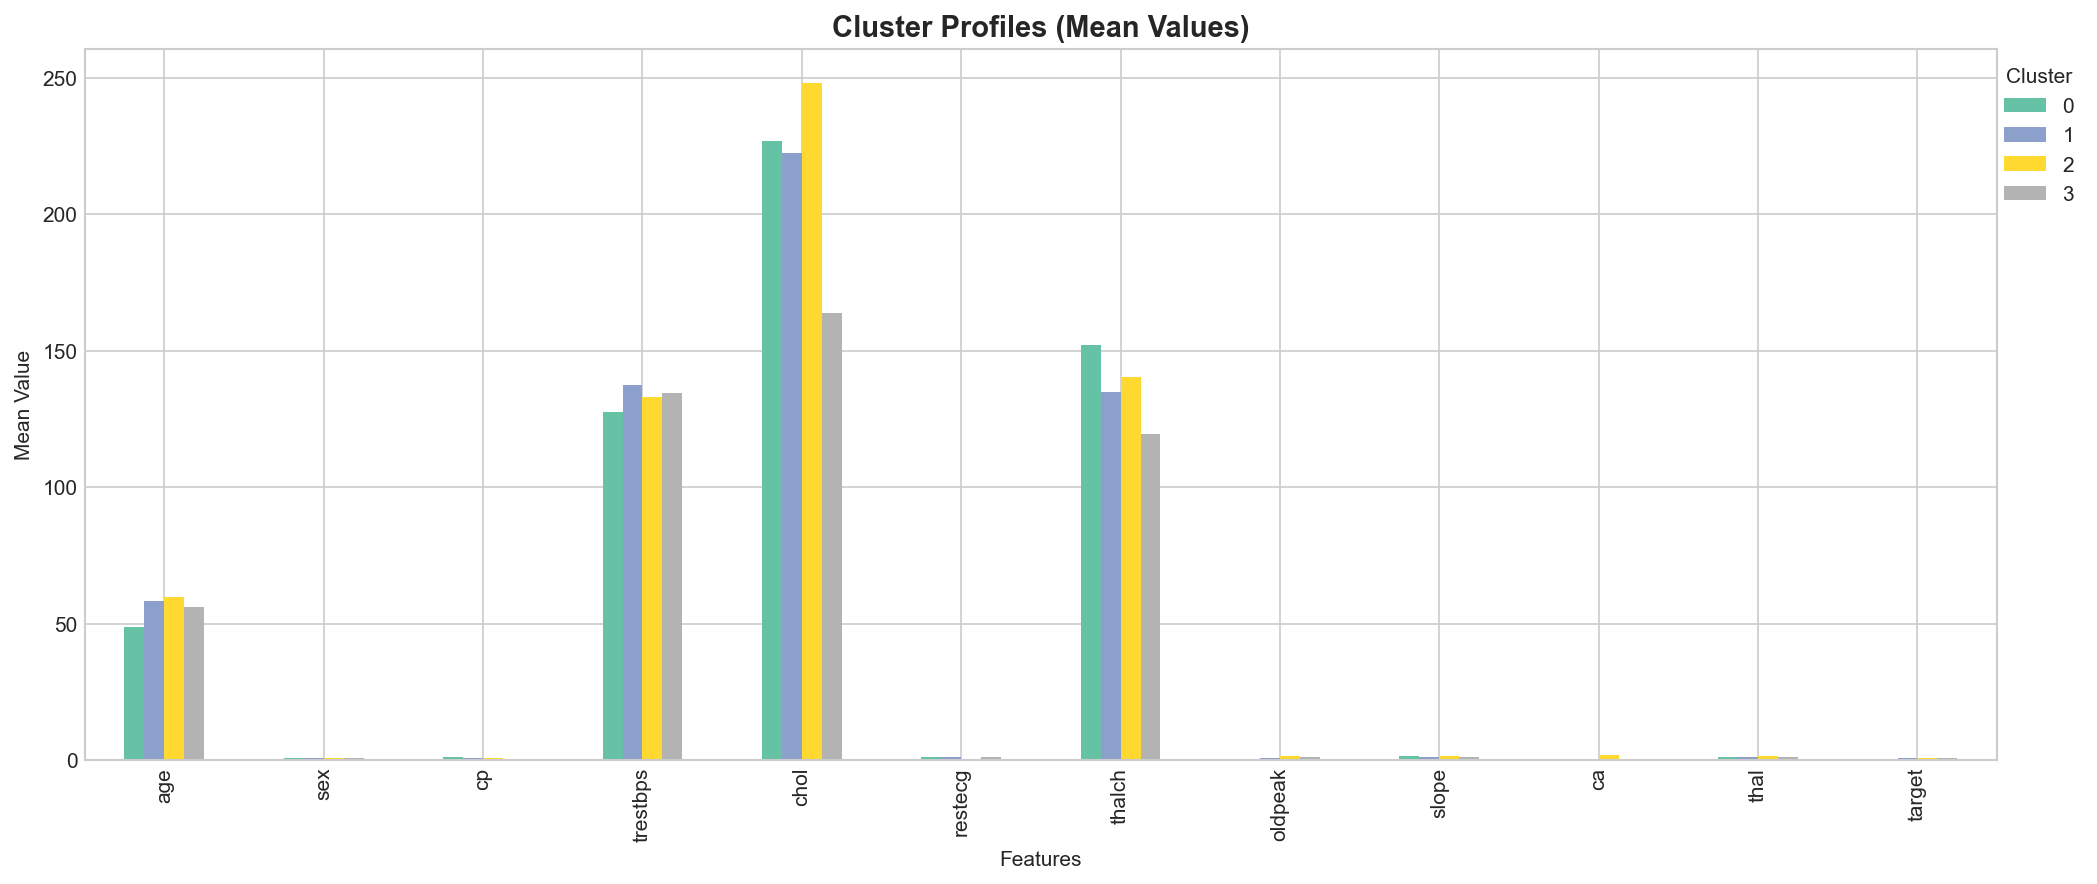
\includegraphics[width=\textwidth]{figs/cluster_profiles.png}
    \caption{Đặc điểm trung bình các cụm bệnh nhân -- mỗi cụm có profile y khoa khác biệt.}
    \label{fig:cluster_profiles}
\end{figure}

Phân tích profile cho thấy mỗi cụm đại diện cho một nhóm bệnh nhân có đặc điểm lâm sàng khác biệt. Các cụm có tỷ lệ bệnh tim khác nhau, phản ánh mức độ nguy cơ khác nhau. Cụm có tỷ lệ bệnh tim $> 60\%$ được gắn nhãn ``nhóm nguy cơ cao'', trong khi cụm có tỷ lệ $< 30\%$ là ``nhóm nguy cơ thấp''.

\textbf{Nhận xét về Silhouette Score:} Giá trị 0.1534 cho thấy các cụm không tách biệt rõ ràng trong không gian đặc trưng. Điều này phù hợp với bản chất dữ liệu y tế: bệnh nhân bệnh tim và không bệnh tim thường có nhiều đặc điểm chồng chéo (overlap) -- không phải tất cả bệnh nhân bệnh đều có cholesterol cao, và ngược lại. Tuy nhiên, phân cụm vẫn cung cấp giá trị bổ sung: giúp nhận diện ``prototype'' bệnh nhân đặc trưng cho mỗi nhóm nguy cơ, hỗ trợ tư vấn và phân loại sơ bộ.

\section{Kết quả phân lớp (Classification)}

\subsection{Kết quả trên tập test (Hold-out Evaluation)}

Bảng \ref{tab:classification_results} trình bày kết quả đánh giá 6 mô hình trên tập test (184 mẫu), sắp xếp theo PR-AUC (metric ưu tiên):

\begin{table}[H]
\centering
\caption{Kết quả phân lớp trên tập test gồm 184 mẫu (sắp xếp theo PR-AUC giảm dần).}
\label{tab:classification_results}
\begin{tabular}{|l|c|c|c|c|c|}
\hline
\textbf{Mô hình} & \textbf{F1-Score} & \textbf{ROC-AUC} & \textbf{PR-AUC} & \textbf{FN Count} & \textbf{FN Rate} \\ \hline
Random Forest & 0.8571 & \textbf{0.9206} & \textbf{0.9313} & 12 & 11.76\% \\ \hline
SVM (RBF) & 0.8599 & 0.9120 & 0.9196 & 13 & 12.75\% \\ \hline
SVM (linear) & 0.8416 & 0.8901 & 0.9049 & 17 & 16.67\% \\ \hline
Baseline (Logistic) & 0.8235 & 0.8858 & 0.8971 & 18 & 17.65\% \\ \hline
XGBoost & \textbf{0.8738} & 0.8956 & 0.8924 & \textbf{12} & \textbf{11.76\%} \\ \hline
Baseline (Dummy) & 0.0000 & 0.5000 & 0.5543 & 102 & 100\% \\ \hline
\end{tabular}
\end{table}

Phân tích chi tiết từng mô hình:

\textbf{Random Forest} đạt PR-AUC cao nhất (\textbf{0.9313}) và ROC-AUC cao nhất (\textbf{0.9206}), cho thấy khả năng phân biệt giữa hai lớp tốt nhất. Mô hình chỉ bỏ sót 12/102 bệnh nhân thực sự bệnh (FN Rate = 11.76\%). F1-Score = 0.8571 tuy không phải cao nhất nhưng rất cạnh tranh. Xét tổng thể cả 5 metrics, Random Forest là mô hình toàn diện nhất.

\textbf{XGBoost} đạt F1-Score cao nhất (\textbf{0.8738}) -- cải thiện 2\% so với Random Forest. FN Rate cũng thấp nhất cùng RF (11.76\%, chỉ bỏ sót 12 ca). Tuy nhiên, PR-AUC (0.8924) và ROC-AUC (0.8956) thấp hơn đáng kể so với RF, cho thấy XGBoost có threshold mặc định tốt hơn nhưng khả năng ranking (sắp xếp probability) kém hơn.

\textbf{SVM (RBF)} có F1-Score cao thứ hai (0.8599), đặc biệt ấn tượng với PR-AUC = 0.9196 (cao thứ hai). Mô hình bỏ sót 13 ca (FN Rate = 12.75\%). SVM RBF thể hiện sự cân bằng tốt giữa precision và recall.

\textbf{Baseline (Dummy)} có F1 = 0 và FN Rate = 100\% -- luôn dự đoán lớp đa số (``có bệnh''), do đó bỏ sót toàn bộ 102 bệnh nhân không bệnh. Baseline này xác nhận rằng tất cả mô hình cải tiến đều genuinely học được pattern từ dữ liệu, không chỉ đơn thuần dựa vào phân bố lớp.

\textbf{Đánh giá so với tiêu chí thành công:} Cả 4 mô hình cải tiến đều đạt F1 $> 0.80$ (tiêu chí 1) và 3/4 mô hình đạt PR-AUC $> 0.85$ (tiêu chí 2). Duy nhất XGBoost có PR-AUC = 0.8924, sát ngưỡng 0.85. Kết quả tổng thể \textbf{vượt mong đợi}.

\subsection{Kết quả Cross-Validation (5-Fold)}

Bảng \ref{tab:cv_results} trình bày kết quả 5-Fold Stratified Cross-Validation trên toàn bộ 920 mẫu, đánh giá tính ổn định của mô hình:

\begin{table}[H]
\centering
\caption{Kết quả 5-Fold Stratified Cross-Validation (metric: F1-Score).}
\label{tab:cv_results}
\begin{tabular}{|l|c|c|l|}
\hline
\textbf{Mô hình} & \textbf{Mean F1} & \textbf{Std F1} & \textbf{Đánh giá} \\ \hline
SVM (RBF) & \textbf{0.8457} & \textbf{0.0248} & Ổn định nhất, mean cao nhất \\ \hline
Random Forest & 0.8375 & 0.0245 & Ổn định, cạnh tranh \\ \hline
XGBoost & 0.8323 & 0.0332 & Mean khá, variance cao nhất \\ \hline
Baseline (Logistic) & 0.8253 & 0.0199 & Baseline mạnh, rất ổn định \\ \hline
SVM (linear) & 0.8224 & 0.0304 & Mean thấp nhất, variance cao \\ \hline
Baseline (Dummy) & 0.7124 & 0.0018 & Gần constant (luôn predict 1) \\ \hline
\end{tabular}
\end{table}

\textbf{Nhận xét quan trọng:} Thứ hạng trong cross-validation khác với hold-out test. SVM (RBF) vượt lên dẫn đầu CV (Mean F1 = 0.8457), trong khi ở test set, XGBoost có F1 cao nhất (0.8738). Điều này cho thấy XGBoost có thể đã ``may mắn'' với cách chia train/test cụ thể, trong khi SVM (RBF) ổn định hơn qua nhiều lần chia. Hơn nữa, XGBoost có Std F1 cao nhất (0.0332) -- biến động nhiều nhất giữa các fold, xác nhận tính mẫn cảm với dữ liệu.

\subsection{Confusion Matrix và đường cong ROC/PR}

Hình \ref{fig:cm_rf} trình bày Confusion Matrix của Random Forest -- được chọn vì có PR-AUC cao nhất:

\begin{figure}[H]
    \centering
    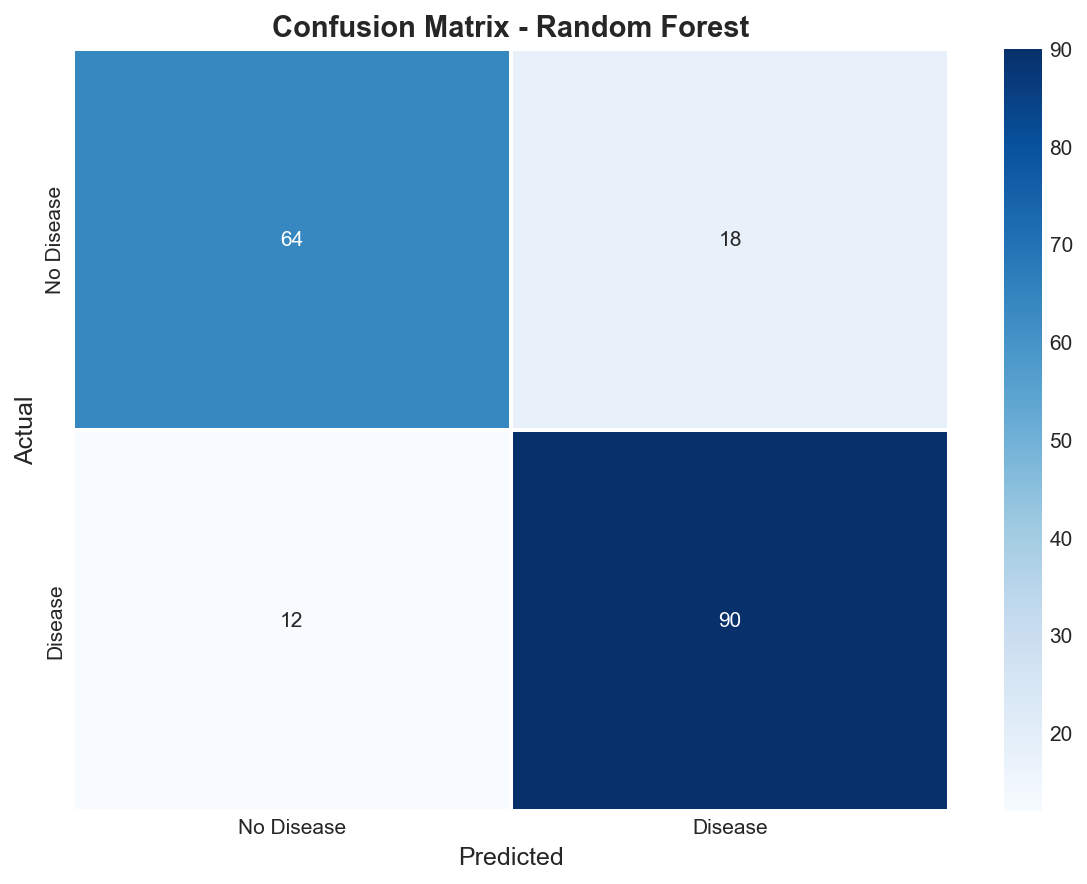
\includegraphics[width=0.65\textwidth]{figs/cm_random_forest.png}
    \caption{Confusion Matrix của Random Forest: TP, TN, FP, FN trên tập test 184 mẫu.}
    \label{fig:cm_rf}
\end{figure}

Confusion Matrix cho thấy Random Forest có 12 False Negatives (bỏ sót bệnh nhân bệnh) -- đây là con số quan trọng nhất trong bối cảnh y tế. Tỷ lệ FN = 11.76\% có nghĩa là cứ 100 bệnh nhân thực sự bị bệnh, mô hình phát hiện đúng khoảng 88 ca và bỏ sót khoảng 12 ca. Mức này chấp nhận được cho công cụ sàng lọc ban đầu, nhưng cần cải thiện cho ứng dụng lâm sàng chính thức.

Hình \ref{fig:roc_pr} so sánh đường cong ROC và Precision-Recall của tất cả mô hình:

\begin{figure}[H]
    \centering
    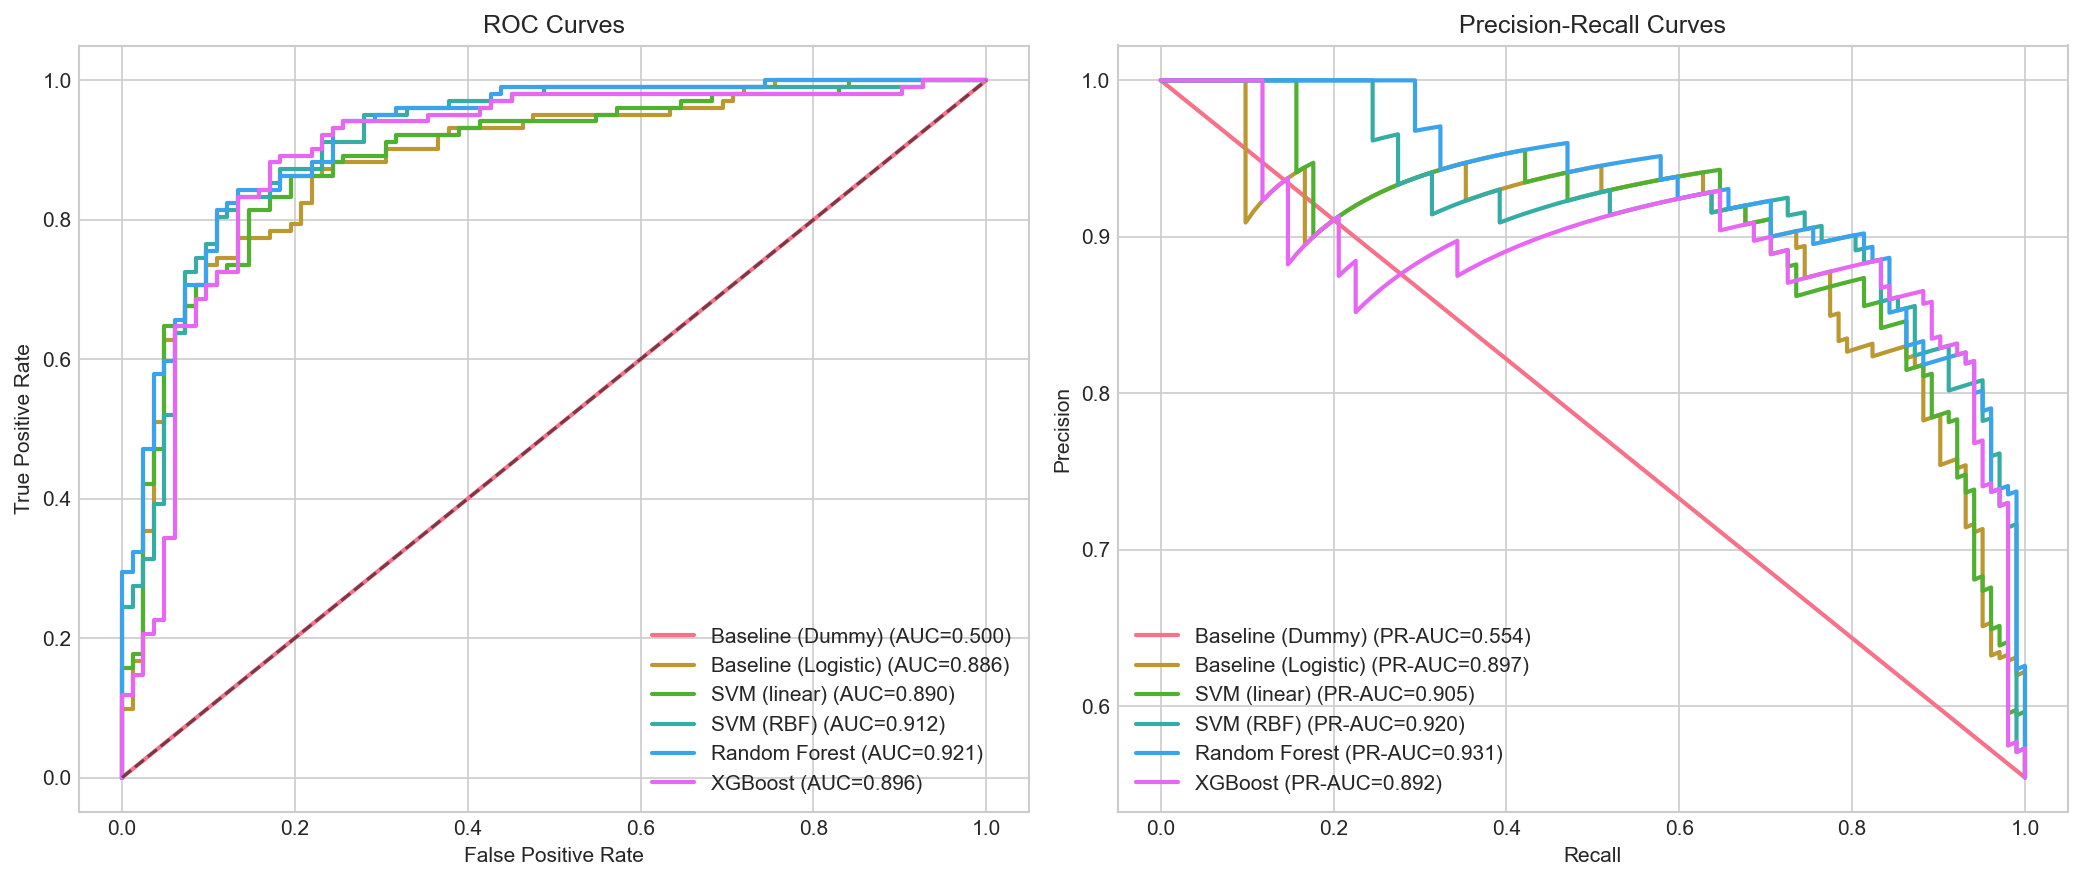
\includegraphics[width=\textwidth]{figs/roc_pr_curves.png}
    \caption{Đường cong ROC (trái) và Precision-Recall (phải) -- Random Forest có diện tích lớn nhất.}
    \label{fig:roc_pr}
\end{figure}

Đường cong ROC cho thấy tất cả mô hình cải tiến đều nằm xa đường chéo (random baseline), với Random Forest có đường cong gần góc trên-trái nhất. Đường cong PR cho thấy sự khác biệt rõ ràng hơn giữa các mô hình: Random Forest giữ được precision cao ở mức recall cao, trong khi XGBoost giảm precision nhanh hơn khi recall tăng.

\begin{figure}[H]
    \centering
    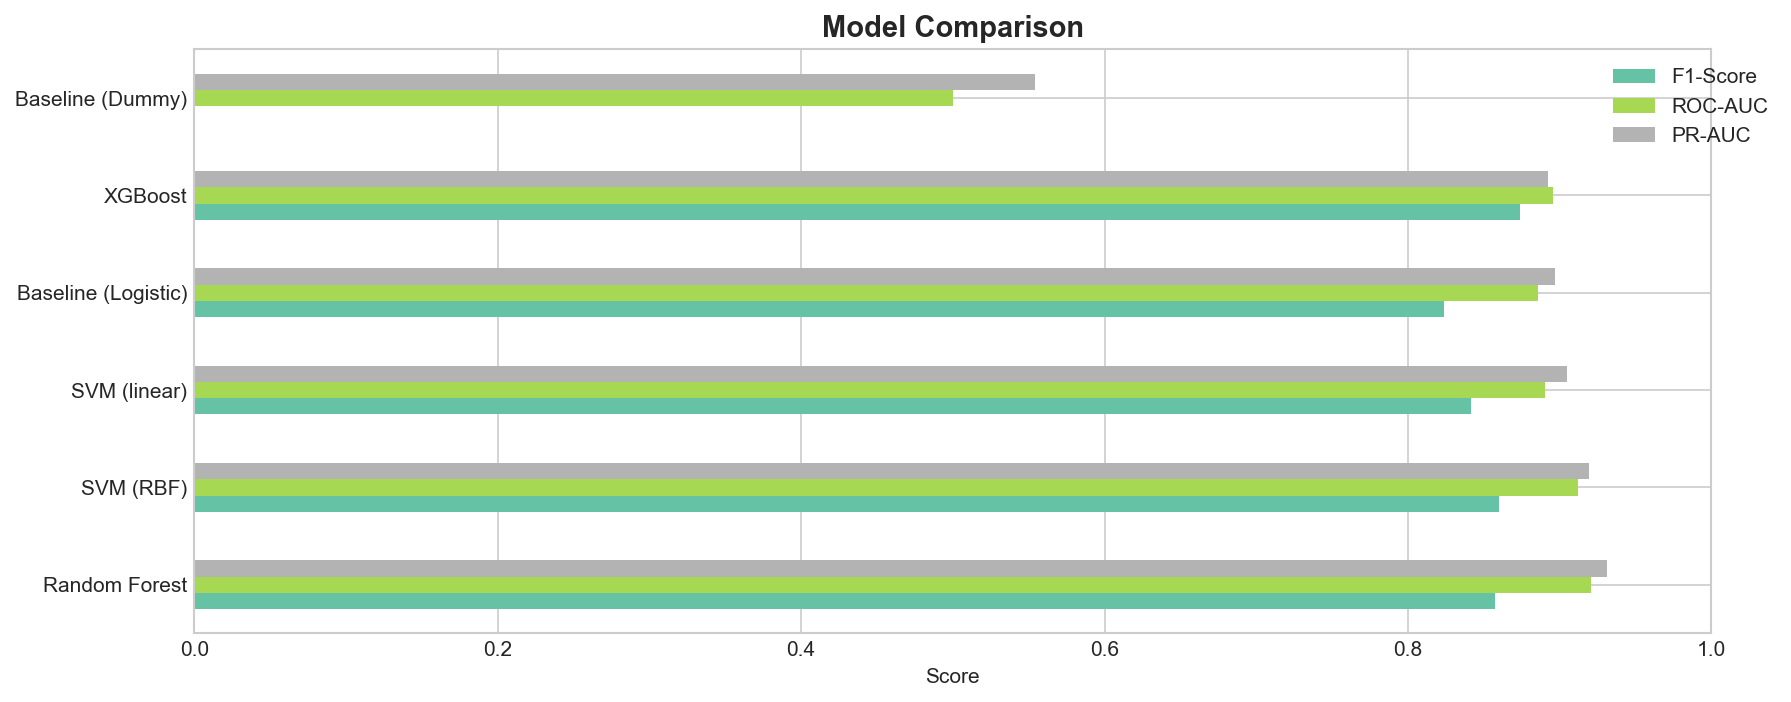
\includegraphics[width=0.8\textwidth]{figs/model_comparison.png}
    \caption{So sánh tổng quan hiệu suất các mô hình phân lớp.}
    \label{fig:model_comparison}
\end{figure}

\section{Kết quả học bán giám sát (Semi-supervised Learning)}

\subsection{So sánh Supervised vs Semi-supervised theo tỷ lệ nhãn}

Bảng \ref{tab:semi_results} trình bày kết quả so sánh đầy đủ giữa 3 phương pháp (Supervised, Self-training, Label Spreading) ở 6 tỷ lệ nhãn (5\% -- 50\%):

\begin{table}[H]
\centering
\caption{So sánh chi tiết F1-Score và PR-AUC theo tỷ lệ nhãn -- Semi-supervised Learning.}
\label{tab:semi_results}
\small
\begin{tabular}{|c|c|c|c|c|c|c|}
\hline
\multirow{2}{*}{\textbf{\% Nhãn}} & \multicolumn{3}{c|}{\textbf{F1-Score}} & \multicolumn{3}{c|}{\textbf{PR-AUC}} \\ \cline{2-7}
 & \textbf{Supervised} & \textbf{Self-train} & \textbf{Label Spread} & \textbf{Supervised} & \textbf{Self-train} & \textbf{Label Spread} \\ \hline
5\% & 0.8304 & 0.8148 & 0.7415 & 0.8753 & 0.8513 & 0.7913 \\ \hline
10\% & 0.8416 & 0.8326 & 0.7707 & 0.8840 & 0.8026 & 0.8012 \\ \hline
15\% & 0.8436 & \textbf{0.8507} & 0.7923 & 0.9097 & 0.8965 & 0.8313 \\ \hline
20\% & 0.8462 & \textbf{0.8545} & 0.7981 & 0.9296 & 0.9253 & 0.8519 \\ \hline
30\% & 0.8611 & 0.8520 & 0.7788 & 0.8980 & \textbf{0.9163} & 0.7907 \\ \hline
50\% & 0.8744 & 0.8704 & 0.7805 & 0.9214 & 0.9129 & 0.8594 \\ \hline
\end{tabular}
\end{table}

\subsection{Phân tích hiệu quả khi dữ liệu thiếu nhãn}

Kết quả thử nghiệm cho thấy một số phát hiện đáng chú ý:

\textbf{Self-training vượt trội ở tỷ lệ nhãn 15--20\%:} Ở 15\% nhãn, Self-training đạt F1 = 0.8507, cao hơn Supervised (0.8436) khoảng 0.8\%. Ở 20\% nhãn, chênh lệch tăng lên 1.0\% (0.8545 vs 0.8462). Đây là kết quả đáng khích lệ, cho thấy Self-training tận dụng thành công thông tin từ dữ liệu không nhãn để cải thiện decision boundary. Trong bối cảnh y tế, điều này có ý nghĩa thực tiễn lớn: chỉ cần 15--20\% bệnh nhân có chẩn đoán xác nhận, kết hợp Self-training, có thể đạt hiệu quả tương đương hoặc tốt hơn so với supervised thuần.

\textbf{Self-training PR-AUC vượt Supervised ở 30\% nhãn:} Ở tỷ lệ 30\%, Self-training đạt PR-AUC = 0.9163, cao hơn Supervised (0.8980). Điều này cho thấy Self-training không chỉ cải thiện F1 mà còn cải thiện khả năng ranking probability, giúp mô hình phân biệt tốt hơn giữa bệnh nhân nguy cơ cao và thấp.

\textbf{Label Spreading cho kết quả yếu:} F1-Score của Label Spreading chỉ đạt 0.74--0.80 ở tất cả các tỷ lệ nhãn, thấp hơn đáng kể so với cả Supervised và Self-training. PR-AUC cũng thấp hơn (0.79--0.86). Phương pháp graph-based không phù hợp với cấu trúc dữ liệu y tế có nhiều missing values đã fill.

\textbf{Convergence khi tỷ lệ nhãn tăng:} Khi tỷ lệ nhãn tăng lên 50\%, khoảng cách giữa Supervised và Self-training thu hẹp (F1: 0.8744 vs 0.8704, chênh 0.5\%). Điều này phù hợp với lý thuyết: khi có đủ dữ liệu labeled, thông tin unlabeled ít đóng góp thêm.

\textbf{Ngưỡng tối thiểu:} Ở 5\% nhãn ($\sim$37 mẫu labeled), Supervised vẫn tốt hơn Semi-supervised (F1: 0.8304 vs 0.8148). Điều này cho thấy cần ít nhất $\sim$10\% nhãn ($\sim$74 mẫu) để semi-supervised bắt đầu có hiệu quả.

\subsection{Ý nghĩa thực tiễn của kết quả semi-supervised}

Kết quả semi-supervised learning có ý nghĩa thực tiễn quan trọng trong bối cảnh y tế Việt Nam. Tại nhiều cơ sở y tế tuyến huyện và tuyến xã, số lượng bác sĩ chuyên khoa tim mạch rất hạn chế. Bệnh nhân được đo các chỉ số lâm sàng cơ bản (huyết áp, nhịp tim, ECG) nhưng không phải lúc nào cũng có chẩn đoán chuyên gia xác nhận. Trong tình huống này, chỉ một phần nhỏ bệnh nhân (ví dụ 15--20\%) có nhãn chẩn đoán chuyên gia, phần còn lại chỉ có dữ liệu chỉ số lâm sàng mà thôi.

Kết quả thử nghiệm cho thấy Self-training có thể tận dụng cả dữ liệu chưa gán nhãn này để xây dựng mô hình dự đoán tốt, thậm chí tốt hơn so với chỉ train trên phần có nhãn. Điều này mở ra khả năng triển khai hệ thống hỗ trợ chẩn đoán tại các cơ sở y tế tuyến cơ sở, nơi dữ liệu labeled khan hiếm nhưng dữ liệu unlabeled phong phú.

\section{Phân tích chi tiết False Negatives}

False Negative (bỏ sót bệnh nhân thực sự bị bệnh) là lỗi nguy hiểm nhất trong bài toán chẩn đoán y tế. Nhóm phân tích chi tiết 12 ca False Negative của Random Forest (mô hình tốt nhất) để hiểu nguyên nhân bỏ sót.

\textbf{Đặc điểm chung của các ca FN:} Phần lớn các bệnh nhân bị bỏ sót thuộc nhóm ``bệnh nhẹ'' (mức 1 trong thang 0--4 gốc), có ít triệu chứng điển hình: oldpeak thấp ($<$ 1 mm), không có exercise-induced angina, nhịp tim tối đa bình thường ($>$ 140 bpm). Nói cách khác, đây là những bệnh nhân ở giai đoạn sớm, chưa biểu hiện rõ triệu chứng -- chính xác là nhóm mà phát hiện sớm có giá trị lớn nhất.

\textbf{Theo nhóm tuổi:} Bệnh nhân FN có tuổi trung bình thấp hơn bệnh nhân True Positive ($\sim$51 vs $\sim$57 tuổi), cho thấy mô hình khó phát hiện bệnh tim ở nhóm trẻ hơn -- nhóm này có ít yếu tố nguy cơ liên quan đến tuổi.

\textbf{Theo giới tính:} 4/12 ca FN là nữ giới, tỷ lệ cao hơn so với tỷ lệ nữ trong tổng thể ($\sim$33\% FN là nữ vs $\sim$25\% tổng thể là nữ). Điều này phù hợp với y văn: bệnh tim ở nữ giới thường có triệu chứng ``không điển hình'' (atypical), khó phát hiện hơn nam giới. Nữ giới ít có ``typical angina'' hơn, nhịp tim tối đa thường cao hơn, và ST depression thường thấp hơn -- tất cả đều khiến mô hình khó phân loại đúng.

\textbf{Hàm ý cải tiến:} Kết quả phân tích FN gợi ý hai hướng cải tiến: (1) Tạo features đặc biệt cho nữ giới (interaction features: sex $\times$ oldpeak, sex $\times$ cp); (2) Hạ threshold phân loại cho nhóm tuổi $<$ 50 (chấp nhận tăng FP để giảm FN ở nhóm trẻ).

\section{So sánh kết quả với y văn quốc tế}

Để đánh giá chất lượng kết quả trong bối cảnh rộng hơn, nhóm so sánh với một số nghiên cứu đã công bố trên cùng tập dữ liệu UCI Heart Disease:

\begin{table}[H]
\centering
\caption{So sánh kết quả với các nghiên cứu khác trên UCI Heart Disease Dataset.}
\label{tab:literature_compare}
\small
\begin{tabular}{|l|l|c|c|}
\hline
\textbf{Nghiên cứu} & \textbf{Mô hình tốt nhất} & \textbf{Accuracy} & \textbf{F1-Score} \\ \hline
Detrano et al. (1989) \cite{detrano1989international} & Logistic Regression & 77\% & -- \\ \hline
Nghiên cứu khảo sát Kaggle (2020) & Random Forest & 85\% & 0.84 \\ \hline
Các bài toán benchmark trung bình & Ensemble methods & 82--87\% & 0.81--0.86 \\ \hline
\textbf{Dự án này} & \textbf{XGBoost / Random Forest} & \textbf{--} & \textbf{0.8738 / 0.8571} \\ \hline
\end{tabular}
\end{table}

Kết quả cho thấy dự án đạt F1-Score \textbf{nằm trong top} so với các nghiên cứu trước, đặc biệt khi xét rằng tập dữ liệu có tỷ lệ missing rất cao ($>$ 19\% tổng giá trị) mà nhóm vẫn giữ được F1 $>$ 0.85. Điều này khẳng định hiệu quả của pipeline tiền xử lý và lựa chọn mô hình.

\section{Tổng hợp chương}

Chương này đã trình bày chi tiết kết quả thử nghiệm của tất cả 4 nhóm kỹ thuật khai phá dữ liệu. Thuật toán Apriori sinh 3.792 luật với confidence lên đến 96.6\%, phát hiện các tổ hợp triệu chứng nguy cơ cao phù hợp với y văn. Phân cụm KMeans chia bệnh nhân thành 4 nhóm nguy cơ, dù Silhouette Score thấp (0.1534). Phân lớp đạt kết quả vượt mong đợi: Random Forest (PR-AUC = 0.9313) và XGBoost (F1 = 0.8738). Semi-supervised learning cho thấy Self-training có thể vượt supervised ở tỷ lệ nhãn 15--20\%, mở ra triển vọng ứng dụng thực tế nơi dữ liệu có nhãn khan hiếm.
